\chapter{Background}
\label{chp:background}
This chapter presents the background and literature on locomotion mode recognition systems for prostheses. The chapter contains seven sections. Firstly background around human gait and prostheses are presented in Sections \ref{sec:background-gait} and \ref{sec:background-Prosthesis}. Following this, Section \ref{sec:background-sensors} reviews wearable sensors used for gait analysis. Sections \ref{sec:background-machine-learning} and \ref{sec:background-ml-lmr} contain an introduction to machine learning and its applications for Locomotion Mode Recognition. Finally, concluding remarks about areas of research interest are presented in Section \ref{sec:background-conclusion}.

%---------------------------------------------%
\section{Biomechanics of Gait}
\label{sec:background-gait}
Gait is a highly individualistic personal trait with many factors that affecting it\cite{Horst2019}. A performant gait is a coherent highly energy-efficient mechanism for forward propulsion of the body. It naturally adapted to different environmental conditions and disturbances to achieve high level of stability throughout the gait cycle\cite{Shah2020, Mummolo2013}. With regards to lower-limb prosthetic the mechanics of locomotion are of most interest. Within this section the terminology that will be used to with reference to the human gait and the high level biomechanics of locomotion are presented.

\subsection{Gait Terminology}
A complete gait cycle is the basic unit of gait analysis. A cycle, by convention, begins when one foot comes into contact with the ground, \acrfull{ic}, and is complete when the same foot contacts the ground again. Another name for \acrshort{ic} is \acrfull{hs}, as the heel is the most common initial point of contact. Conversely, the point at which the foot leaves the ground is \acrfull{to}. The name arises as the toe is always the last point of contact with the ground.\cite{Novacheck1998, Shah2020}

The gait cycle can be further sub-divided into two phases. The distinct phases, stance and swing, are physically indicated by the foot's contact with the ground. Stance occurs when the foot is in contact with the ground, and swing occurs when the foot is off the ground. \acrshort{hs} marks the transition from swing to stance and \acrshort{to} stance to swing. When considering both limbs, there are additional descriptors. These include single support when only one foot is in contact with the ground and double support when both feet are in contact with the ground. Figure \ref{fig:background_gait_cycle} illustrates a complete gait cycle and the key events.\cite{Novacheck1998, Shah2020}

% Picture of gait cycle indicating key events
\begin{figure}[!hbt]
    \centering
    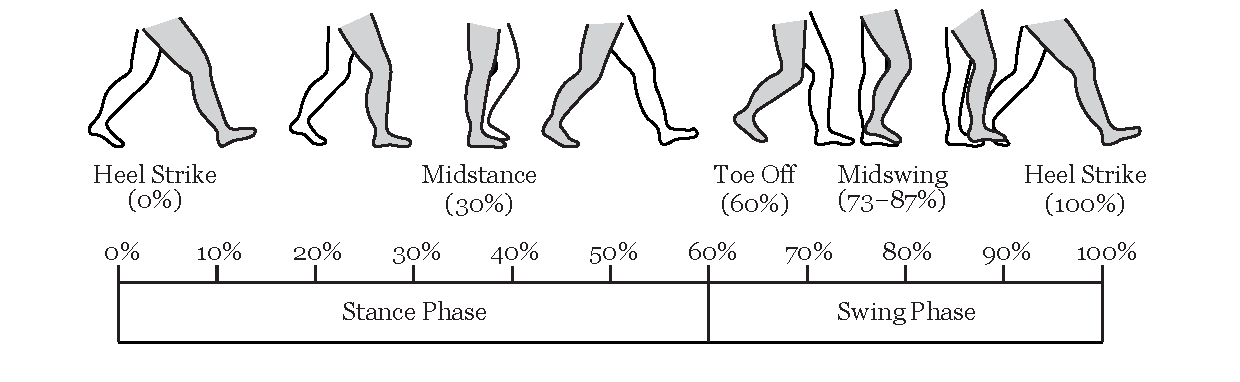
\includegraphics[width=\textwidth]{content/4-LSTM_Behaviour/Gait_Cycle.pdf}
    \caption[Human Gait Cycle during level walking]{Human Gait Cycle during level walking. The percentage timings of the gait events are approximate; they vary depending on the individual and environment.\cite{Sherratt2021}}
    \label{fig:background_gait_cycle}
\end{figure}

Movements of the human body mainly occur in three planes, sagittal, frontal/mediolateral and horizontal/transverse. The plane's intersections occur either at a joint centre or the body's \acrfull{com}. The sagittal plane is the vertical plane passing from the rear (posterior) to the front (anterior), dividing the body left and right. The mediolateral plane passes from left to right, dividing the body into posterior and anterior halves. The transverse plane divides the body into the top (superior) and bottom (inferior) halves.\cite{Bartlett2007} Figure \ref{fig:background_planes_of_the_body} shows an illustration of the three planes

% Image of different planes of human motion
\begin{figure}[!hbt]
    \centering
    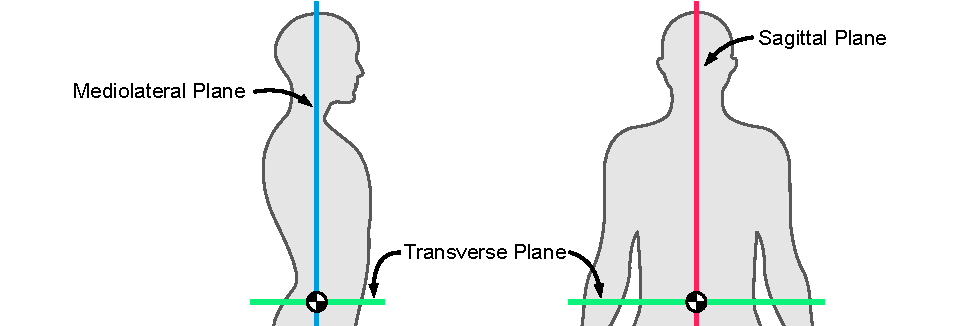
\includegraphics[width=0.9\textwidth]{content/2-Background/body_planes.pdf}
    \caption[Bio-mechanical planes of the body]{Bio-mechanical planes of the body. The sagittal plane is the vertical plane dividing left and right body halves. The mediolateral plane divides the body into front and rear halves. Finally, the transverse plane divides the body into the top and bottom halves.}
    \label{fig:background_planes_of_the_body}
\end{figure}

The primary movement of the ankle occurs in the sagittal plane; these are the raising and lowering of the foot. The two motions are plantar-flexion, moving the foot downwards, and dorsiflexion, lifting the foot upwards.\cite{Bartlett2007} Figure \ref{fig:background_plantar_dorsi_flexion} show a visual of the ankle movement.  Plantar-flexion happens towards the end of the stance phase when the foot pushes off the ground. Dorsiflexion occurs during the early swing phase to provide enough toe clearance as the foot passes under the body.\cite{Whittle2012}

\begin{figure}[!hbt]
    \centering
    
\includegraphics[width=\textwidth]{content/2-Background/Ankle_Flexion.pdf}
    \caption[Sagittal plane motions of the ankle]{Sagittal plane motions of the ankle. Plantar flexion is the lowering of the foot; dorsiflexion is the raising of the foot.}
    \label{fig:background_plantar_dorsi_flexion}
\end{figure}

There are many different metrics for quantifying gait. These vary from easily measurable values such as step rates and distances to more involved metrics such as energy expenditure and efficiency.\cite{Ramakrishnan2019, Coutts1999}.

%---------------------------------------------
\subsection{Variation with Locomotive Activity}
The previous section described the pattern of gait that occurs during a level walking locomotion. The human gait cycle can efficiently adapt to different terrain and obstacles. Everyday locomotive activities include climbing stairs and walking up and down sloped surfaces in built-up environments. Changes in the locomotive activity require a change in gait actions to accomplish the movement. Additional muscle actions are required to raise and lower the \acrshort{com} during these actions\cite{Franz2012a}.

This section presents the difference between five different locomotive movements, Walking, \acrfull{sa}, \acrfull{sd}, \acrfull{ra}, \acrfull{rd}. Ramps are considered any surface with a slope sufficiently steep so that a change in locomotive action is required. For each activity, there is a description of the differences in human gait compared to walking.

\paragraph{Stair Ascent} During \acrshort{sa}, the \acrshort{com} must move upwards, requiring net positive work; this requires more significant muscle activity. \acrshort{sa} can be divided into three phases: weight acceptance, pull-up and forward continuation. The knee dominates during weight acceptance and pull-up with support from the hip and ankle. While, during forward continuation, the ankle generates a large amount of energy resulting in an upwards motion of the \acrshort{com}. The ankle angle differs from a horizontal walk, mainly at the late swing phase and early stance. While lifting the foot to the next tread, the edge is avoided by a small dorsiflexion and moving the knee backwards.\cite{Svensson2007}

\paragraph{Stair Descent} During \acrshort{sd}, the ankle angle differs from horizontal in the swing phase when moving the limbs down. The change in ankle angle is most notable as a dorsiflexion action to reaching the toe downwards. The change in ankle angle results in the toe being the point of \acrshort{ic}. Energy is transferred from the ankle into the knee at \acrshort{ic}. Due to the downwards, \acrshort{com} motion reflects in a smaller force at push-off. There is also less muscle activity for vertical movements due to the smaller stride length.\cite{Svensson2007}

\paragraph{Ramp Ascent} As with \acrshort{sa}, \acrshort{ra} requires additional energy expenditure to move the \acrshort{com} upwards\cite{Franz2012a}. Walking uphill can take three times as much energy as walking on flat ground\cite{Matsumoto2017}. Gait parameters also vary with the slope of the surface\cite{Kimel-Naor2017}. Knee flexion and ankle dorsiflexion increases at heel strike as the foot aligns with the surface. These changes in gait require an increased range of motion and additional muscle power generation.\cite{McIntosh2006}

\paragraph{Ramp Descent} For moderate slopes, \acrshort{rd} is similar to level walking. However, the lowering of the \acrshort{com} requires additional energy to be absorbed\cite{Franz2012a}. Walking downhill takes only half as much energy as walking on the level ground\cite{Matsumoto2017}. As with \acrshort{ra}, the gait adjusts to the slope.

The above describes the steady-state motions during typical locomotive activities. The human gait can also smoothly transition between different locomotive modes and handle perturbations and disturbances.\cite{Li2019}



%---------------------------------------------%
\section{Lower Limb Prosthesis}
\label{sec:background-Prosthesis}
A lower-limb amputation involves the removal of part, or multiple parts, of the lower limb. The practice of amputation for injury or disease is centuries old and likely first occurred in pre-historic times\cite{Kirkup2007}. The level of amputation can be either minor or major, depending on the amputation site. Major lower limb amputations occur above the ankle. The two most common major lower limb amputations are trans-femoral (above the knee) and trans-tibial(below the knee).

An artificial or prosthetic limb can replace an amputated extremity. The prosthesis aims to restore natural behaviour by emulating/augmenting the action of a missing limb.\cite{Tucker2015} The ability of a prosthesis to mimic the function and appearance of the lost limb can vary significantly.

Amputee gait is asymmetrical and different from that of a non-amputee, amputees relying more heavily on their unaffected side.\cite{Bateni2002, Varrecchia2019} In the absence of ankle plantar flexor power, hip extensors and flexors, as well as hip external rotators, become the major power generators. In contrast, the primary absorption source becomes hip abductors, adductors, and knee extensors. Increased hip extensor activity was observed for the sound limb, accompanied by less hip abduction-adduction activity.\cite{Sadeghi2001}

Studies have shown that trans-tibial amputees using passive prosthesis use 10-40\% more energy to walk at the same speed when compared to their non-amputee peers\cite{McDonald2018, Herr2012}, with trans-femoral amputees requiring more than 70\%\cite{Stewart2008}. This additional energy expenditure dramatically impedes ambulation, where amputees are half as active as their non-amputee peers and prefer 30-40\% slower walking speeds\cite{Bussmann2008, Piazza2017, Lin2014, Au2009}. The loss of significant power generating muscles after amputation also leads to a marked asymmetry in gait between limbs\cite{Button2010}.

The earliest known prostheses are recorded in Indian literature between 1500 to 800 b.c. although artificial limbs are probably much older than that\cite{Breakey1976}. Over the years, prostheses have gone from barely functional to sophisticated devices aiming to replicate lost functionality. Artificial limb design, fitting and manufacture has advanced considerably within the past 50 years and is now a burgeoning research field.\cite{Kirkup2007}

% Types of prosthetic
The current primary technologies for prosthetic legs are; \acrfull{esr}, hydraulics, semi-active and active devices\cite{Asif2021}. Figure \ref{Fig:CH2-prostheses_type} shows examples for each type.

\begin{figure}[!hbt]
\centering
  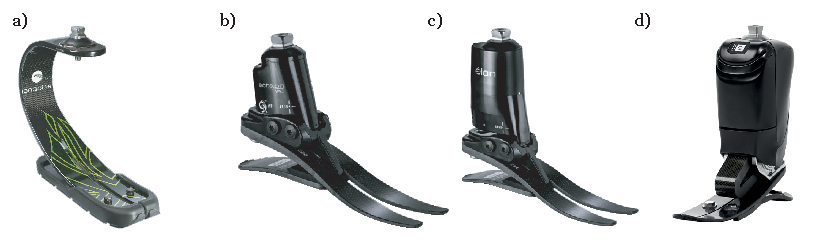
\includegraphics[width=\textwidth]{content/2-Background/ch2_prosthetic_device_types.pdf}
  \caption[Example prostheses types]{Example prostheses types: a) ESR (Blatchford BladeXT), b) Hydraulic (Blatchford EchelonVAC), c) Semi-active (Blatchford Elan), d) Active (Ottobock's biOM) (a-c)\cite{blatchford2018} (d)\cite{biom2018} }
  \label{Fig:CH2-prostheses_type}
\end{figure}

Each technology offers varying levels of assistance, with amputee suitability and preference informing selection. The most common form of prostheses is the \acrshort{esr} foot. During walking, an ESR prosthesis reduces energy expenditure by storing energy through spring compression during heel loading, releasing it during late stance to push-off.\cite{Asif2021}

Passive devices such as an \acrshort{esr} cannot provide the net positive mechanical power needed during many activities of daily living, such as ascending stairs or standing up from a seated position\cite{Simon2013}. To fully restore gait functionality, the prostheses must replace the lost power generating function of the amputated limb.

A powered active prosthetic device could provide the full power-output capabilities of the corresponding physiological joints. It could thus enable gait patterns resembling those of unaffected persons across various activities and terrain\cite{Tucker2015, Bhakta2020}. According to Au et al., The use of an active prosthetic can reduce metabolic energy usage by 14\% in trans-tibial amputees, even with a two-fold increase in prosthetic weight\cite{Au2009}.

Ottobock's BiOM EmPOWER active prosthetic ankle is currently the only active prosthetic device on the market.\cite{Nayak2020} The device is a spin-out from research undertaken by MIT in 2011.\cite{biom2018} Analysis of the EmPOWER ankle has shown a reduction in the metabolic cost of walking by 8\% and an increased walking velocity of 23\%\cite{Herr2012}.\ {\"O}ssur produces the Proprio Foot, a semi-active ankle that lifts the toe to increase ground clearance. The Proprio foot has also been integrated with their Rheo Knee to form a coordinated leg for trans-femoral amputees capable of stair descent.\cite{Ossur}

% ----------------------------------
\subsection{Control Requirements for Powered Prosthesis} % Introduce the problem
The human body represents a well-balanced walking machine that performs periodic, stable, and energy-efficient gait through highly sophisticated mechanics and control, which are not easy to replicate\cite{Mummolo2013}. The human nervous system uses different control strategies to adapt to individual locomotive activities\cite{Lay2007, Simon2013}. These adaptations occur automatically in a healthy gait cycle. A prosthetic controller must implement multiple control modes to replicate this lost functionality.

To effectively control an active prosthetic device several concurrent processes have to be implemented. Tucker et al. present a generalised hierarchical framework for structuring a prostheses controller, see Figure \ref{Fig:lit-rev-controller_framework}. Hardware state control forms the lowest level. The top level contains implementation of a perception system to determine user intent or activity mode. Translation of intent to hardware state control is performed by a intermediate level.\cite{Tucker2015}

An active prostheses controller must implement several concurrent processes to control prostheses effectively. Tucker et al. present a generalised hierarchical framework for structuring a prostheses controller. Hardware control forms the lowest level. The top-level controller implements a perception system to determine user intent or activity mode. Therefore, an accurate perception of the users' intended action is paramount\cite{Asif2021, Hernandez2021}. An intermediate level controller performs translation of intent to hardware state demands. An illustration of the hierarchical controller is provided in figure \ref{Fig:lit-rev-controller_framework}.\cite{Tucker2015}

\begin{figure}[!hbt]
\centering
  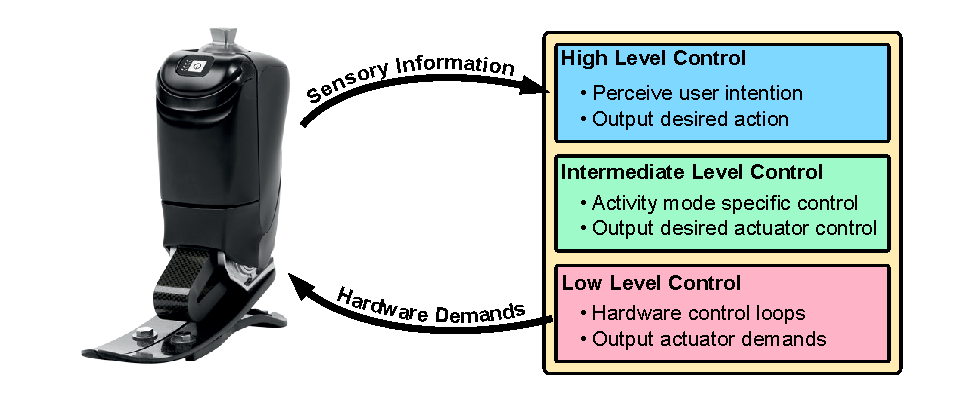
\includegraphics[width=\textwidth]{content/2-Background/control_hierarchy.pdf}
  \caption{Generalised control framework for active lower limb prostheses}
  \label{Fig:lit-rev-controller_framework}
\end{figure}


%---------------------------------------------%
\section{Sensors}
\label{sec:background-sensors}
To perceive a person's intent, we must take measurements of them\cite{Asif2021, Hernandez2021}. Different sensors allow for different measurements. Each measurement can be of physical quantities about the person or their surrounding environment. Appropriate selection of sensors is therefore of critical importance. Criteria for selection include the type, richness of information and impact on the user.\cite{Tucker2015}

The impact of a sensor considers its invasiveness both physically and in privacy. The physical impact must consider how the discomfort of a sensor affects the performance of an action. For example, a sensor of fewer than 300 grams mounted to a shoe does not affect gait significantly\cite{AbdulRazak2012}. In contrast, many wires rubbing on the leg may. There are also practical concerns, such as ease of use.

Sensing systems divide into three categories: neural, mechanically intrinsic or environmental signals. Neural sensors measure physiological electrical signals, such as brain activity or muscle activity. Mechanically sensors measure effects intrinsic to the device itself, such as acceleration. Environmental sensors measure the properties of the world around them, such as ambient light or pressure.\cite{Koller2018, Tucker2015}

Recent trends in sensing technology have been towards wearable sensors. The demands of the modern smartphone have primarily driven this development. New smaller and more precise sensors have opened up the possibility for making previously lab bound measurements in a more natural environment. Smartphone sensing technology is highly applicable and widely used in active prostheses\cite{Asif2021}; this state of the art review will focus only on wearable technologies.

% Mechanical signals
Acceleration and angular velocity are the most commonly mechanically intrinsic signals measured. A wide variety of wearable sensors can collect this information.\cite{Shull2014, Tucker2015} Acceleration and angular velocity are the most commonly mechanically intrinsic signals measured. A wide variety of wearable sensors can collect this information. Other common wearable sensors include goniometer and inclinometers for angular displacements, and pressure transducers or Force Sensitive Resistors (FSR) for foot loading and initial/terminal contact points. Ground Reaction Force (GRF) can also be measured using pressure transducers such as an FSR\cite{Schepers2007}.

The most common wearable sensor used is the \acrfull{imu}\cite{Shull2014}. An \acrshort{imu} is a single integrated circuit containing a three-axis accelerometer and a three-axis gyroscope. The development of smartphones has dramatically reduced the sensors' cost, precision, and size. When an IMU includes a three-axis magnetometer, the sensor becomes a \acrfull{marg} sensor. Using one or multiple sensors allows the determination of limb or joint orientation, angular velocities and accelerations. 

Smartphones commonly contain \acrshort{imu}s and other sensors. Their onboard sensing and integrated nature have made them popular data collection platforms\cite{Garcia-Gonzalez2020, Mutegeki2020}.

% Neural
Neural signals provide a more natural interface for controlling prosthesis\cite{He2018} but pose significant challenges in there use. Neural sensors detect muscle control signals conversely mechanically intrinsic measure the effect of muscle force. Therefore, neural signals can be detected earlier, tens of milliseconds\cite{Tucker2015}, giving longer to perform classification. However, their output is often challenging to interpret. Mechanical signals are often more straightforward to measure due to their lower impact and greater tolerance to placement and conditions.\cite{Koller2018} ElectroMyoGraphy (EMG) is the most common technique, electric potential produced by skeletal muscle activity is measured through electrodes attached to the muscle on interest.

% Environmental
The environment around the user can provide context to local sensor data. Different environments increase the likelihood of encountering a particular terrain feature.\cite{Tucker2015, Tschiedel2020} Jin et al. investigated a wearable environmental sensing package to augment other activity and location recognition methods. Jin evaluated three sensors temperature, humidity, and ambient light. They measured repeatable changes in sensor data during different activities, for example, a temperature drop due to airflow over the sensor package during motion.\cite{Jin2014} Fu et al. also investigated an environmental sensor. The wearable sensor package used contained a barometric pressure sensor allowing for changes in altitude to be detected\cite{Fu2021}.

% Placement
The placement of sensors is an important consideration; the chosen location should maximise the richness of data while minimising invasiveness\cite{Tucker2015}. Shull et al. reviewed the location of wearable sensors for gait analysis. Most articles identified used sensors sensitive in the mediolateral axis, with the knee, trunk and shank the most popular sensing location.\cite{Shull2014}

The prosthetic device is the obvious mounting location providing a rigid and stable sensor platform for prosthetic users. Attachment is more challenging for biological limbs; temporary attachment of sensors by medical tape or elastic strapping is common. Consideration for changing the shape of the limb during movement is required.

Where suitable muscles are present at the skin, electrodes can be attached to the skin's surface above the muscle. Surface EMG presents the least invasive technique for the neural sensory system. However, they must be attached securely to the body to prevent artefacts from corrupting sensor movement readings and require individual calibration.


%---------------------------------------------%
\section{Machine Learning}
\label{sec:background-machine-learning}
% Overview of machine learning aim and operation
\acrfull{ml} is a subset of computer science that focuses on systems that learn from data. An \acrshort{ml} system can numerically estimate a complex function from exposure to examples of a phenomenon. That is to say, an \acrshort{ml} algorithm can convert experience into expertise or make predictions from data. As an entirely numerical approach, it is especially compelling for problems of high dimensionality. There are many different tasks where machine learning can be powerfully used, such as classification, translation, denoising and synthesis.\cite{Mitchell1997, Shalev-Shwartz2014, Goodfellow2015, Burkov2019}

What separates machine learning from optimisation is that we want to minimise the task error not only for the seen experience but also for novel unseen inputs. Minimising the task error forms the crux of machine learning.\cite{Goodfellow2015}

% What is the machine learning process
The machine learning process usually follows three steps; 1) gathering a representative data set; 2) building a model to solve the task based on knowledge captured in the data set; 3) testing and evaluating model performance\cite{Burkov2019}. The output is a model that encapsulates the learnt knowledge. The model is deployable in the real world to perform the taught task.\cite{Shalev-Shwartz2014}.

% How is experience provided
By gathering knowledge from experience, \acrshort{ml} avoids the need to formally specify all knowledge to accomplish a task\cite{Goodfellow2015}. This approach significantly reduces the implementation burden and may enable previously intractable solutions for highly complex systems. Experience is provided as a set or sets of examples of the input and often the corresponding output or label. The set of examples is called the training data.

The model input for each example is a feature vector. Each element of a feature vector contains one quantitative measure of the example. Each feature is either handpicked, such as the mean of a signal, or learnt where raw data is fed directly into the model learnt. The choice of data representation or features can heavily affect the performance of a machine learning system. Handpicking features are labour intensive and without care can result in bias in the machine learning model. However, learnt features require more data for training and are harder to control.\cite{Bengio2013}

The quality of the training data is essential to good learning, as by the adage garbage, in garbage out. However, data quality measurements can be challenging because they must consider qualitative factors such as realism.

The training data is used at various stages throughout the learning process to provide knowledge and verify system performance. The whole training data is split into three sets. Training – a set of examples from which the system learns. Validation – a set used to evaluate the generalisation performance during training. Test – used to evaluate the final generalisation performance after training. 

% How is experience converted to knowledge - training/optimisation
Most \acrshort{ml} algorithms involve optimisation of some form. Optimisation refers to the task of either minimising or maximising some function. The function we want to optimise for is called the criterion. The criterion measures what a good prediction is. When minimising the criterion, the criterion is often called the cost or loss function.\cite{Goodfellow2015} The learning algorithm uses the criterion to optimise model weights and biases to incorporate knowledge from the training data.

% Types of training
There are four standard techniques for Machine Learning: supervised, unsupervised, semi-supervised, and reinforcement learning. Each is useful for different tasks and require different forms of experience.

Supervised learning uses a labelled dataset to produce a model that can deduce the correct output from a given input\cite{Burkov2019}. In unsupervised learning, the training data set is unlabelled. The system is left to discover variation and beneficial properties across the data set. Semi-supervised learning lies between supervised and unsupervised. Some but not all example inputs have labels. The algorithm uses known inputs to label unknown examples to build a more extensive labelled training set\cite{Abdallah2018} Reinforcement learning does not experience a fixed dataset. Instead, they interact with an environment using feedback to learn.

% Transfer learning
An additional form of learning is transfer learning. The research field of transfer learning is concerned with the reapplication of captured knowledge. The application changes can be significant, visually identifying a new object, or minor, such as personalisation to an individual. Many schemes exist for achieving knowledge transfer. Schemes include fine-tuning part or all of a model, extending an existing model with additional layers or generating a mapping to adapt a new input source.\cite{Farahani2020, Zhuang2021}

% How is performance measured
Understanding the final performance of the trained model requires additional metrics as the loss function is often not directly interpretable. These quantitative metrics represent the \acrshort{ml} system's ability to perform the desired task. Often the metric will be directly inheritable, such as the proportion of examples where the output was correct. The performance metric is generally evaluated for all three data sets to evaluate different aspects of model performance. For example, generalisation, or the performance for unseen data, can be evaluated using the test set.

% Other aspects of machine
Many issues may occur while developing an \acrshort{ml} system. For example, over/under-fitting. Fitting problems occur when the model either learns too tightly to the training set or cannot learn the desired task. Therefore it cannot predict new unseen inputs. Adjustments to the learning rate, training data or training time will affect fitting. Adjustments to system hyper-parameters control properties such as these. Any settings determined outside the learning algorithm are called hyper-parameters.\cite{Goodfellow2015}

% How are machine learning models constructed
Many \acrshort{ml} models exist and have been used widely across many different tasks.. Some typical machine learning models are Random Forest, \acrfull{svm}, \acrfull{mlp} (Dense when fully connected), \acrfull{cnn}, \acrfull{rnn}.

\acrshort{mlp}, \acrshort{cnn} and \acrshort{rnn} are all forms of \acrfull{ann}. They are referred to as networks because they are typically implemented by composing together many different functions. The neural aspect comes from the original inspired by replicating biological neurons. Modern-day systems are often not biologically inspired.

Multiple layers of units neurons form an \acrshort{ann}. The layer location in the neural network determines its name. The first network layer that receives input data is called the input layer. The network's last layer is called the output layer for similar reasons. The intermediate layers are hidden layers. By adding more layers and more units within each layer, a network can represent functions of increasing complexity\cite{Goodfellow2015}.

Each layer in a neural network is composed of many cells or units. The cell's make-up depends on the type of layer. The connections between cells are also dependent on the layer type. All cells have at least one feed-forward connection to the next layer. A fully connected layer is where each cell connects to every cell on the next layer. When forward feed networks include feedback connections, they are called \acrshort{rnn}s.

Two common ML architectures are \acrshort{cnn}s and \acrshort{rnn}s. The CNN is a specialised neural network that use convolution to combine inputs. They are well suited to grid-like data such as images or regular sampled time-series data. This architecture has been successful in practical applications, primarily visual problems.\cite{Goodfellow2015}

The RNN is a family of neural networks for processing sequential data. Their structure allows them to process longer sequences than practical for other networks.\cite{Goodfellow2015} The most common form of RNN used is the Long Short Term Network (LSTM). The LSTM resolves some of the issues with training a standard RNN through additional methods of information flow control\cite{Hochreiter1997}. \acrshort{lstm}s can learn temporal dependencies better by efficiently remembering valid predictors from past inputs and forgetting unnecessary artefacts\cite{Hernandez2021}.



%---------------------------------------------%
\section{Machine Learning for Locomotion Mode Recognition}
\label{sec:background-ml-lmr}
Classifying human activities from sensor data is challenging. The signal difference between activities is often subtle and highly individualised.\cite{Zhu2019} Machine learning methods are well suited to this task, and consequently, have been widely adopted\cite{Wang2019b}.

% How would ML be useful to prosthesis?
Outside machine learning activity classifiers use heuristic methods. The heuristic is usually a fixed set of rules that controls the transition between activities modes. Heuristics methods are the current standard for modes selection in powered prostheses\cite{Varol2008, Lawson2014, Gorsic2014, Young2014a}. Individual tuning is required to achieve adequate performance; the manual nature of this process makes it challenging to scale\cite{Tucker2015}. Machine learning methods offer the potential to achieve better, more personalised performance with less manual input\cite{Hernandez2021, Zhu2019, Rai2019a}.

% How can machine learning be useful for activity recognition
Researchers have produced many machine learning architectures for solving \acrshort{har} problems. Typically, \acrshort{har} \acrshort{ml} models all follow the same structure. A window of sensor data is collected and fed directly into the model. This direct approach improves the signal-to-noise ratio\cite{Hernandez2021}. The model classifies the activity producing the corresponding output.% Figure \ref{fig:back-sensor-based-deep-learning} illustrates this structure.\cite{Wang2019b}

% \begin{figure}
%     \centering
%     \includegraphics[width=0.6\textwidth]{example-image-duck}%{content/2-Background/sensor-based-deep-learning.png}
%     \caption[An illustration of sensor-based activity recognition using a machine learning approach]{An illustration of sensor-based activity recognition using a machine learning approach\cite{Wang2019b}.}
%     \label{fig:back-sensor-based-deep-learning}
% \end{figure}

%------------------------------------------ NOT WRITTEN YET -----------------------------------%
% Types of machine learning models
Most researchers developing machine learning processes for \acrshort{har} use a supervised learning approach\cite{Saini2020, Straczkiewicz2021}, with only a few examples of unsupervised and semi-supervised learning\cite{Bota2019}.

Locomotive data is usually continuous time series in nature. The continuous sensor data must be split and labelled with the current activity for supervised learning methods. The most common form of this is to use a sliding window that divides continuous data into chunks. The activities encompassed by the window determine its label.

A large number of papers use \acrfull{cnn} and \acrfull{lstm} networks to implement \acrshort{har}. Both network types are well suited to regularly sampled sensor data. 

\acrshort{cnn} architectures use convolutional and pooling layers to extract features from the sensor data. A dense \acrshort{mlp} layer forms the final classification based on the outputs from the final \acrshort{cnn} layer. \cite{Jiang2015, Lu2020, Martinez-Hernandez2021} 

Rae et al. has shown that\acrshort{rnn} networks adjust well to subject-specific variations\cite{Rai2019a}. \textbf{rnn} ahas been used frequently for \acrshort{har} problems, most commonly implemented using \acrshort{lstm} unit. The layer structure of \acrshort{rnn} networks is such that the output of each \acrshort{lstm} unit layer is fed only into the \acrshort{lstm} units at the same timestep. The formation of final classification uses either all the outputs of the last layer or only the last set of units.\cite{Yu2018, Uddin2021a}

Recently researchers have begun combining \acrshort{cnn} and \acrshort{lstm} networks to form Deep Convolutional and \acrshort{lstm} networks\cite{Ordonez2016}. The convolutional layers are placed either as the input or just before the output.\cite{Mutegeki2020, Xia2020}


% How is this useful for amputees?
Only a few papers have applied \acrshort{ml} techniques to the problem of \acrshort{imu}-based \acrshort{lmr} classifiers for amputees. Of them, only three papers have tested their methods on amputee gait data\cite{Lu2020, Bruinsma2021, Jamieson2021}. The lack of testing on amputees is likely due to the difficulties of collecting gait data from amputees\cite{Gardiner2016}.

Bruinsma et al. tested different configurations of \acrshort{rnn} and \acrshort{cnn} networks. Gait data from a trans-femoral amputee was collected. The amputee wore two \acrshort{imu}s mounted on the thigh and shank. All collection of gait data was in a controlled environment. The gait data did not include any non-amputees subjects for comparison. Evaluation of different network architectures revealed that the \acrfull{gru} and \acrshort{lstm} networks performed highest, achieving greater than 80\% accuracy. The best performance of  93.06\% occurred when using a \acrshort{gru} network fed with data from both \acrshort{imu}s.\cite{Bruinsma2021}

Su et al. demonstrated \acrshort{cnn} classifiers with both amputees and non-amputees. Su produced a dataset collected in a controlled environment to test the classifiers. Ten non-amputee and a single trans-tibial amputee were asked to walk up and down a single staircase, ramp, and flats. Both a general classifier tested with a subject not used for training and a bespoke classier trained and tested with data from a single individual were tested. The bespoke classifier performed as highly, achieving an average performance of $94\%$ for the ten non-amputees and $89\%$ for the single trans-tibial amputee. The results of the general model showed a drop in performance to an average of $82\%$. It is not clear if this number includes performance using the trans-tibial amputee.\cite{Su2019}

Jamieson et al. developed and evaluated the performance of a general \acrshort{lstm} classifier trained using data from non-amputee. They collected a dataset of \acrshort{imu} gait data from eight non-amputees and four subjects with lower limb amputation. Each subject wore a single hip worn \acrshort{imu} as they walked an improvised route through a natural environment. Performance testing of the \acrshort{lstm} classifier showed that when classifying non-amputees, performed was adequately at $78\%$. However, when presented with an amputee, performance dropped dramatically to an average of $28\%$.\cite{Jamieson2021}

Bespoke models can achieve good classification performance for individuals, including amputees. However, there is still significant room for improvement of \acrshort{imu}-based LMR classifiers. The difficulty in collecting amputees' data limits research in this area and the practicality of deploying a developed system. Therefore any system that can leverage knowledge from other more obtainable sources would be highly advantageous. None of the three studies into amputees have publicly released their data.


%---------------------------------------------%
\section{Conclusions}
\label{sec:background-conclusion}
Gait is a highly individual trait. The human body has evolved to use distinct control modes for accomplishing different locomotive actions. Lower limb amputees have many gait difficulties. For a lower limb prosthetic device to fully restore the lost functionality, it must be powered and replicate the different control modes. Part of the challenge of achieving this is determining the locomotive intent of a subject.

Machine learning has made significant inroads in identifying human activities from low-cost \acrshort{imu}s likely to be present on powered lower limb prostheses. However, limited research has occurred in machine learning techniques for human activity recognition of lower limb amputees. The lack of research is likely due to the difficulties of collecting gait data from amputees. Research into ways to reduce the data requirements for \acrshort{imu}-based locomotion mode recognition systems for lower limb prosthesis is required.
